%----------------------------------------------------------
% Experimental Evaluation
%\label{sec:key-impact}
%----------------------------------------------------
%\subsection{Evaluation workflow}
%\section{Conversation Quality Evaluation System}
\label{sec:CQAS}
%\subsection{Conversational Quality Assessment Problem}
\begin{figure}[tp]  
\centering % Still centering the figure  
\hspace*{-1cm} % Shift the entire figure to the left by 1 cm  
\resizebox{0.90\columnwidth}{!}{ % Keep the size slightly below the full column width for better fit  
\tikzstyle{root} = [rectangle, fill=white!3, text width=4.5em, text centered, minimum height=2em, node distance=.10cm]  
\tikzstyle{block} = [rectangle, draw, fill=blue!3, text width=5.3em, text centered, minimum height=2em, node distance=.40cm]  
\tikzstyle{block1} = [rectangle, draw, fill=red!3, text width=7em, text centered, minimum height=2em, node distance=.5cm]  
\tikzstyle{block2} = [rectangle, draw, fill=gray!3, text width=6em, text centered, minimum height=2em, node distance=.5cm]  
\tikzstyle{block3} = [rectangle, draw, fill=green!10, text width=8em, text centered, minimum height=2em, node distance=.55cm]  
\tikzstyle{line} = [draw, -latex']  
  
\begin{tikzpicture}[auto, node distance=2cm,>=latex']  
    % Place nodes  
    \node [root] (root1) {};  
    \node [block1, right=of root1] (interactions) {\texttt{\textbf{AGREE-Dog}} User-System Interactions};  
    \node [block2, below=of interactions] (history) {Recording Metrics Automatically};  
    \node [block2, right=of history] (lemma) {Model-Repair Log Files};  
    \node [block2, right=of lemma] (quality) {Conversation History Management};  
    \node [block3, above=of quality] (stat) {\textcolor{blue}{Statistical Analysis and Visualization}};  
  
    % Draw edges  
    \path [line] (root1)  (interactions);  
    \path [line] (interactions) -- (history);  
    \path [line] (history) -- (lemma);  
    \path [line] (lemma) -- (quality);  
    \path [line] (quality) -- (stat);  
\end{tikzpicture}  
} % End of resizebox  
\caption{AGREE-Dog Conversation Quality Assessment Workflow (CQAW). The workflow tracks structural metrics from conversation histories and temporal metrics from copilot logs, leveraging timestamps to measure user and LLM response latencies. Finally, metrics are analyzed and visualized using AGREE-Dog's statistical utility}  
\label{fig:CQAS}  
\end{figure}



\subsection{Evaluation Setup and Fault Injection Protocol}

Using the Conversation Quality Assessment Workflow (CQAW, Figure~\ref{fig:CQAS}), we systematically tracked structural and temporal metrics to comprehensively evaluate AGREE-Dog. Our experiments involved thirteen fault-injected test scenarios based on an AADL-based Car model. Each scenario featured dynamically evolving artifacts—including AADL source files, natural-language requirements, counterexample traces, AGREE log files, and LLM-generated diagnostics—culminating in approximately 32,100 tokens across all scenarios. On average, scenarios began with around 400 lines of AADL and log content, fewer than 100 lines of counterexample traces, and less than 100 lines of natural-language inputs.

Faults targeted three safety-critical subsystems (Top-Level Control, Steering, and Transmission), triggering 16 repair cycles. Injected faults covered typical behavioral and contract-level violations—ranging from incorrect assumptions, logic errors, and range violations to faulty assignments and temporal inconsistencies. Repairs were accepted only after passing AGREE's formal verification and manual user confirmation via AGREE-Dog’s \texttt{insert} command, ensuring both correctness and soundness. Detailed scenarios and artifacts are documented in Appendix~\ref{appendix:test-scenarios} and made available in our public GitHub repository\footnote{\url{https://github.com/loonwerks}}.

\begin{figure}[t]
  \centering
  \caption{AGREE-Dog Evaluation Metrics and Convergence}
  \label{fig:agree-metrics-combined}

\begin{subfigure}{\textwidth}
    \centering
    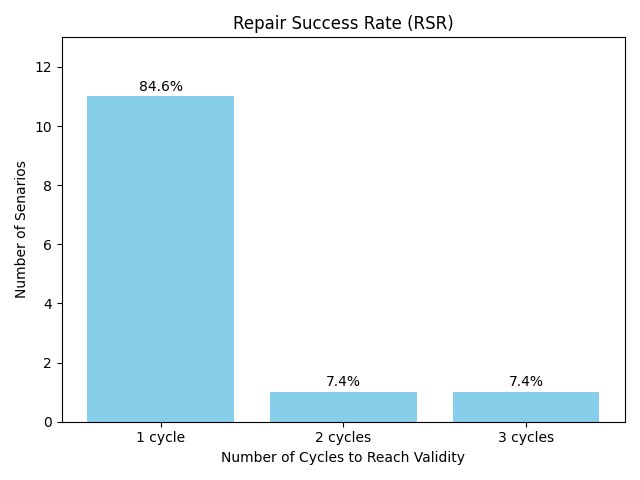
\includegraphics[width=0.6\linewidth]{repair-histogram.png}
    \caption{Repair cycles required to achieve system-wide validity.}
    \label{fig:repair-histogram}
  \end{subfigure}

  \vspace{1em}
  
  \begin{subfigure}{\textwidth}
    \centering
    \caption*{(b) Structural and Temporal Metrics Summary}
    \begin{minipage}{\textwidth}
      \centering
      \begin{tabular}{@{}p{0.48\textwidth} p{0.45\textwidth}@{}}
        \toprule
        \textbf{Metric} & \textbf{Result} \\
        \midrule
        \multicolumn{2}{l}{\textit{Structural Metrics}} \\
        System Validity & 100\% achieved for all test scenarios\\
        Repair Success Rate (RSR) & 11/13 (84.6\%) in 1 cycle; 1/13 in 2 cycles; 1/13 in 3 cycles \\
        Human Input Ratio (HpR) & $<$ 0.1\% of total tokens \\
        AGREE-Dog Generated Input & $>$ 99.9\% of total tokens \\
        Token Use (per test suite) & 4.8k, 5.5k, 22k tokens \\
        \addlinespace
        \multicolumn{2}{l}{\textit{Temporal Metrics}} \\
        Wall-Clock Time (WCT) & Mean: 2:09 min; Median: 1:39 min \\
        LLM Latency (per cycle) & Mean: 22 s; Range: 4--33 s \\
        \bottomrule
      \end{tabular}
    \end{minipage}
  \end{subfigure}

\end{figure}


\subsubsection*{Evaluation Metrics.}
Figure~\ref{fig:repair-histogram} visualizes repair convergence across the scenarios. Table~\ref{fig:agree-metrics-combined} summarizes AGREE-Dog’s structural and temporal performance metrics (defined in Section~\ref{sec:metrics}).  Next, we highlight key findings that emerged during the experiment.
%%%%%%%%%%%%
\subsection{Key Results.}
This evaluation demonstrates the feasibility of integrating generative AI (GenAI) with formal verification in Model-Based Systems Engineering (MBSE). By combining large language model reasoning with AGREE-based validation in OSATE\,2, AGREE-Dog delivers verifiable repairs with minimal human effort. %Below, we highlight key findings that emerged during the experiment.

\begin{enumerate}
%
\item \textbf{Rapid Convergence with Reduced Human Intervention Frequency:}
AGREE-Dog resolved approximately 85\% (11 out of 13) of the test cases within a single cycle, while the remaining cases required two or three cycles (approximately 7.5\% each). This demonstrates swift convergence and significantly reduces the frequency of user interventions needed across diverse fault scenarios.

\item \textbf{High Automation with Minimal Human Effort:}
Estiamted by (HpR) metric, Human-generated content constituted less than 0.1\,\% of the overall tokens, with AGREE-Dog autonomously generating more than 99.9\,\% via its integrated prompt construction mechanism and language model. Combined with the rapid convergence rate noted previously, this outcome highlights AGREE-Dog’s capability to effectively automate model repairs, significantly reducing manual input relative to the extensive verification contexts encountered.

\item \textbf{Efficiency and Reduced Human Return Time (HRT):}

AGREE-Dog demonstrated significant computational and cognitive efficiency throughout the evaluation. Internal computational overhead consistently remained below one second per operation, complementing an average LLM latency of approximately 22 seconds per cycle. While the median overall wall-clock time (WCT) was about 1 minute and 39\,s the average human response time (HRT) was approximately 1 minute and 3 seconds. This average, however, was notably skewed by two outlier cases; in fact, 85\,\% of scenarios achieved total resolution (WCT) in under 45 seconds—including LLM latency—limiting human analysis and decision-making time to less than 23 seconds per scenario in 11 out of 13 cases. Compared to traditional manual verification approaches, which typically require hours or days, AGREE-Dog’s structured guidance and intuitive natural-language explanations significantly reduced human cognitive effort estimated by (HRT) metric and the overall interaction duration (WCT). %The absence of noticeable performance degradation further indicates the potential to effectively scale AGREE-Dog to more complex scenarios, although such expansions might necessitate advancements in memory management, refined context selection strategies, recommendation mechanisms, or targeted model fine-tuning.
\end{enumerate}
%\textbf{Memory-Informed Reasoning.} In one case, the system recalled a previously used strategy (diffing) and reused it to generate the correct fix on the first attempt—evidence of contextual awareness.


%%%%\subsubsection{Summary of main observation}
%%The evaluation provides clear evidence that integrating generative AI (GenAI) with formal verification tools such as AGREE can substantially enhance model repair workflows within Model-Based Systems Engineering (MBSE).
%
%%Using diverse test scenarios totaling approximately 32,000 tokens—realistically spanning thousands of artifact lines—AGREE-Dog consistently maintained logical coherence, formal validity, and user efficiency. 
%
%%These results offer strong support for the effectiveness of this approach, particularly on smaller-scale models. 
%
%%Given recent advances such as GPT-4.1's expanded context window (up to 1 million tokens), these outcomes are very encouraging, motivating further exploration into applying this neuro-symbolic approach to more complex, industrial-scale formal verification tasks.
%%We break down the key observations,:


